\documentclass[12pt, a4paper]{article}
\usepackage{iem} %enthaelt viele nuetzliche usepackages und definiert 
% ein paar Reformatierungen
\hyphenation{}

\begin{document}
\selectlanguage{ngerman}

\title{Untersuchung verschiedener Upmixingmethoden für DirAC}

\author{Manuel Planton, BSc \\ Michael Hirschmugl, BSc\\\\\small{Betreuung: Dr. Franz Zotter, Dr. Matthias Frank}}

\markboth{}{M. Planton, M. Hirschmugl: DirAC Upmixing}

\doctype{Seminararbeit aus Algorithmen in Akustik und Computermusik 2}

%\date{Juni 2008}

\maketitle
\newpage
\pagestyle{empty}
\hspace{1cm}\vspace{3cm}

\hspace{1cm}\vspace{1cm}

\begin{abstract}
   Kurzfassungstext. Beispielzitate Buch~\cite{Williams}, in einem Konferenzband\cite{Avizienis06}, Diplomarbeit~\cite{Pomberger08}, Dissertation~\cite{Li05}, Fachzeitschriftenartikel~\cite{Weinreich80}.
\end{abstract}
\newpage
\pagestyle{myheadings}
\hspace{1cm}\vspace{2cm}

\tableofcontents
\newpage

\section{Einleitung}

\section{DirAC}
    \subsection{Implementierung}
    In diesem Abschnitt wird beschrieben, wie der DirAC-Algorithmus in diesem Projekt implementiert wurde. Die Implementierung liegt als Script für GNU Octave vor und nutzt das \textit{signal}-Package. Der Code dafür ist zu großen Teilen direkt dem Buch \textit{Parametric Time-Frequency Domain Spatial Audio} ~\cite{spatial-book} von V. Pulkki entnommen.

\paragraph{Übersicht}
Zu Beginn des Skriptes wird das Eingangssignal im B-Format erster Ordnung eingelesen. Dieses muss als \textit{.wav}-Datei vorliegen und genau vier Kanäle (in der Reihenfolge $w$, $x$, $y$, $z$) umfassen. Die Samplerate wird direkt aus dieser Datei ermittelt und als Variable \textit{fs} im Workspace von GNU Octave gespeichert.

Anschließend wird eine Liste von Lautsprecherpositionen eingelesen. Dabei handelt es sich entweder um die Anordnung des einhüllenden Wiedergabesystems (z.B. 12 Lautsprecher im Produktionsstudio des IEM Graz), oder eine allgemeine t-Design Anordnung (in diesem Fall 48 Punkte für ein 9-Design). Die Koordinaten werden in sphärische Richtungen umgerechnet und daraus eine dreidimensionale VBAP-Matrix berechnet. Die Anzahl der Spalten dieser Matrix entspricht der Anzahl der eingelesenen Positionen (12 oder 48). Die Zeilenanzahl ist abhängig von der gewählten Richtungsauflösung (= 1 Grad). Diese Matrix dient dazu, gerichtete Audiosignale auf die Ausgabekanäle (reale Lautsprecheranordnung oder allgemeines t-Design) abzubilden.

Im nächsten Schritt wird eine Dekodierungsmatrix von virtuellen Mikrofonen erzeugt, um die vier Eingangskanäle $w[n]$, $x[n]$, $y[n]$ und $z[n]$ des B-Format-Signals auf die Ausgangskanäle (12 oder 48) dekodieren zu können. Dabei wird eine Supernieren-Charakteristik eingesetzt.

Das B-Format Eingangssginal wird anschließend in einer Schleife in zeitlichen Blöcken (Fenster) verarbeitet. Ein Fenster besteht dabei aus jeweils 512 Samples und wird in einer 1024-Punkt Fouriertransformation mit der Hilfe der Funktion \textit{fft()} in den Frequenzbereich transformiert. Die FFT-Länge wurde als doppelte Blocklänge gewählt um Aliasing zu vermeiden. Die zeitlichen Blöcke werden noch mit einem Hann-Fenster für die Resynthese beaufschlagt. Ein Hann-Fenster kann in Octave mit der Funktion \textit{hann()} (alternativ: \textit{hanning(), abgeleitet von ``to hann''}) erzeugt, und einfach als Vektor mit den Zeitsignalen multipliziert werden.
        \paragraph{Analyse von Richtungs- und Diffusanteil}
        Zur Bestimmung von Richtungs- und Diffusanteil werden zunächst Schallschnelle und Energie berechnet. Die Schnallschnelle wird als Vektor $\textbf{V}_{m}[k] = [X_{m}[k], Y_{m}[k], Z_{m}[k]]$ aus den gerichteten Anteilen (der Druckgradienten-Mikrofone) des B-Format Signals bestimmt. Der Schalldruck ist der omnidirektionale Anteil $W_{m}[k]$. Die Indizes $m$ und $k$ werden hier zur Kennzeichnung des Zeitfensters als Funktion der Frequenzzahl $k$ verwendet.

Der Pseudo-Schallintensitätsvektor $\textbf{I}_{m}[k]$ wird aus dem Schnellevektor und dem konjugiert komplexen Schalldruck in Gleichung \ref{eq:inten} abgeleitet, wobei hier rein der Realteil heranzogen wird, da sonst die Blindeinteile des Schnellevektors das Ergebnis verfälschen würden \cite{pulkki}. Der Intensitätsvektor stellt bereits die Schalleinfallsrichtung für alle Frequenzbins einzeln dar, jedoch entgegengesetzt der Einfallsrichtung $\textbf{D}_{m}[k]$

\begin{equation}
    -\textbf{D}_{m}[k] = \textbf{I}_{m}[k] = \Re(W_{m}[k]^{*} \cdot \textbf{V}_{m}[k]) .
    \label{eq:inten}
\end{equation}

Die Schallenergie $E_{m}[k]$ wird mit Hilfe der Gleichung

\begin{equation}
    E_{m}[k] = \frac{|W_{m}[k]|^2+||\textbf{V}_{m}[k]||^2}{2}
    \label{eq:energy}
\end{equation}

ausgewertet.

Um Sprünge in der Lautsprecherzuordnung von gerichteten Signalen bei raschen Bewegungen zu vermeiden, wird der Intensitätsvektor zusätzlich durch eine zeitliche Mittelwertbildung geglättet. Diese Glättung kann im Skript mit einer frequenzabhängigen Zeitkonstante vorgegeben werde. Zusätzlich wird auch der Energievektor zeitlich geglättet. Anschließend wird der Intensitätsvektor verwendet, um die Einfallsrichtungen in sphärischen Koordinaten zu bestimmen.

Die Diffusität $\psi_{m}[k]$ kann schlussendlich aus dem Vergleich des Betrags des Intensitätsvektors mit der Energie ermittelt werden

\begin{equation}
    \psi_{m}[k] = \sqrt{1 - \frac{||\mathbb{E}(\textbf{I}_{m}[k])||}{\mathbb{E}(E_{m}[k])}} .
    \label{eq:diff}
\end{equation}

 Der Erwartungswert entspricht hier den (zeitlich) gemittelten Vektoren.

%\begin{figure}[!ht]
%  \centering
%  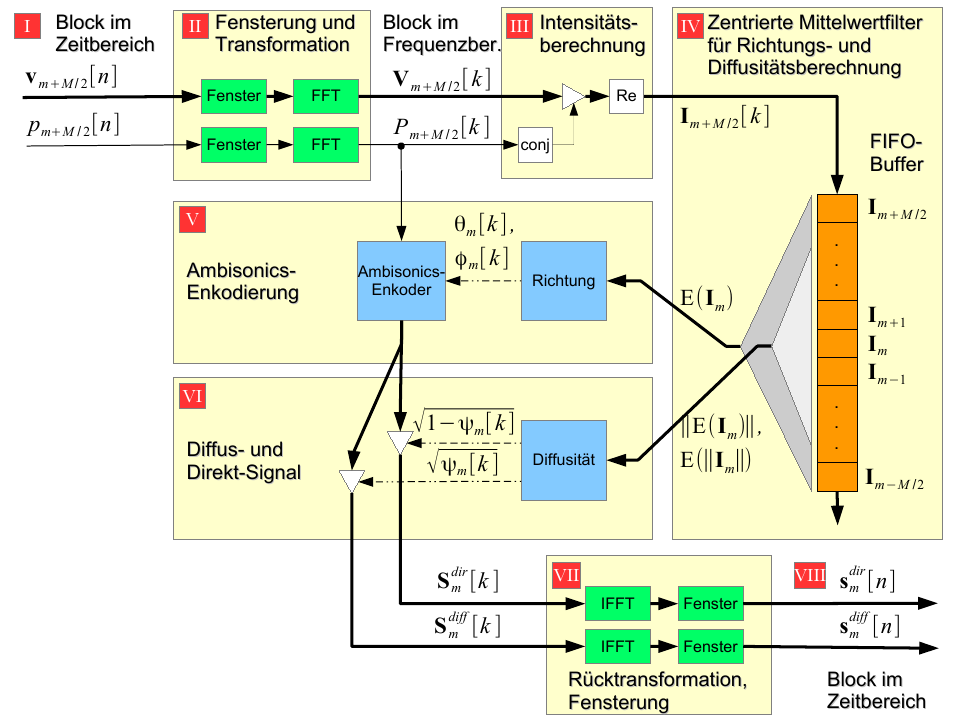
\includegraphics[width=0.7\textwidth]{implementierung/plots/flow.png}
%  \label{fig:flow}
%  \caption{Flussdiagram des DirAC Algorithmus in Octave \cite{seminar2016}}
%\end{figure}
        \paragraph{Upmixing auf Lautsprecherandordnung}
        

%Zur Dekodierung auf eine bestimmte Lautsprecheranordnung wird eine Matrix aus virtuellen Mikrofonen berechnet, woraus sich eine Tabelle mit Gain-Werten ergibt. Diese Tabelle besteht aus einer Spalte für jeden Lautsprecherkanal und kann die einzelnen Frequenzbins in einem VBAP-Verfahren den enstprechenden Lautsprechern zuordnen. In dieser Seminararbeit wurden dabei zwei Ansätze für die Dekodierung verglichen: Einerseits die direkte Dekodierung auf die physische Lautsprecheranordnung des Wiedergabesystems, und andererseits ein allgemeiner Ansatz womit die Dekodierung auf eine t-Design Lautsprecheranordnung erfolgt. Dieser Dekodierungsansatz hat den Vorteil, dass die Wiedergabeanordnung zum Zeitpunkt des Upmixings nicht vorgegeben sein muss. Auch für die Klangqualität ergeben sich daraus Vorteile, welche im Hörversuch besprochen werden.

Im Frequenzbereich wird jeder Spektralblock mit dem Sampling-Dekoder dekodiert, um die vier Eingangskanäle in eine höhere Kanalzahl zu wandeln.
In dieser Seminararbeit wurden dabei zwei Ansätze für die Dekodierung verglichen: Einerseits die direkte Dekodierung auf die physische Lautsprecheranordnung des Wiedergabesystems, und andererseits ein allgemeiner Ansatz womit die Dekodierung auf ein t-Design erfolgt. Dieser Dekodierungsansatz hat den Vorteil, dass die physische Lautsprecheranordnung zum Zeitpunkt des Upmixings nicht gegeben sein muss.

Bei einem 9-Design (Abb. \ref{fig:tdesign_image}) ergibt sich eine sphärische Anordnung von 48 virtuellen Lautsprechern, welche eine optimale dekodierung des B-Formats erlaubt.

\begin{figure}[!ht]
  \centering
  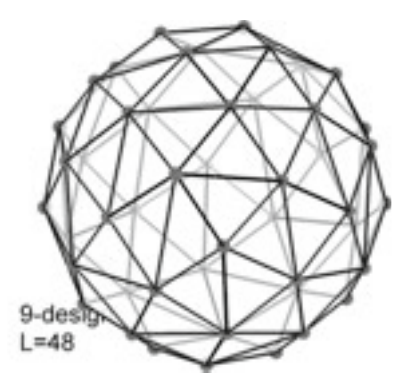
\includegraphics[width=0.35\textwidth]{implementierung/plots/t-design.png}
  \caption{9-Design T-Design \cite{ambi-book}}
  \label{fig:tdesign_image}
\end{figure}

%Zur Dekodierung wird in Octave also eine Matrix mit Lautsprechergewichten für Schalleinfallsrichtungen erstellt. Somit kann einer gegebenen frequenzabhängigen Richtung (bestehend aus Azimuth und Elevation), ein bestimmter Gain-Wert am entsprechenden Lautsprecherkanal zugeordnet werden.

        \paragraph{Trennung von Diffus- und Richtungsanteil}
        %Die Trennung von Diffus- und Richtungsanteil erfolgt im Frequenzbereich, wobei beide Anteile aus dem omindirektionalen Anteil des B-Format Signals durch gewichtete Filterung erzeugt werden. Prinzipiell wird für den gerichteten Anteil ein spektraler Block im Frequenzbereich mit zwei Matrizen multipliziert: Einerseits mit der VBAP-Tabelle um die Richtung einem Lautsprecher zuzuordnen, und andereseits mit dem ebenfalls frequenzabhängigen Diffusitätsvektor. Somit werden Frequenzbins mit frequenzabhängigen Diffusitätswerten gewichtetet, und diesen anschließend entsprechende Lautsprechergewichte zugeordnet.

%Nach der Berechnung des gerichteten Signalanteils kann auch der Diffusanteil aus dem omnidirektionalen Signal erzeugt werden. Dieser entspricht lediglich dem nicht-gerichteten Anteil des omnidirektionalen Signals und wird daher aus der Filterkurve des Direktanteils bestimmt. Somit ergeben sich an dieser Stelle zwei frequenzabhängige Signalmatrizen für Diffus- und Richtungsanteil. Beide Matrizen besitzen eine Spalte für jeden Lautsprecherkanal und die Zeilenzahl entspricht der FFT-Länge.

Die Trennung von Diffus- und Richtungsanteil erfolgt ebenfalls im Frequenzbereich. Der frequenzabhängige Diffusitätsvektor wird hier verwendet, um den gerichteten Anteil aus den dekodierten Signalen (mit 12 oder 48 Kanälen) zu filtern. Prinzipiell wird für den gerichteten Anteil ein spektraler Block mit zwei Matrizen multipliziert: Erstens mit dem frequenzabhängigen Diffusitätsvektor, und weiters mit der VBAP-Tabelle um die gerichteten Signale den entsprechenden Lautsprechern zuzuordnen. Somit werden Frequenzbins mit frequenzabhängigen Diffusitätswerten gewichtetet, und diesen anschließend entsprechende Lautsprechergewichte verliehen.

Nach der Berechnung des gerichteten Signalanteils kann auch der Diffusanteil aus den dekodierten Signalen erzeugt werden. Dieser entspricht dem nicht-gerichteten Anteil und wird daher aus der Filterkurve des Direktanteils bestimmt. Somit ergeben sich an dieser Stelle zwei frequenzabhängige Signalmatrizen für Diffus- und Richtungsanteil für jedes zeitliche Verarbeitungsfenster. Beide Matrizen besitzen eine Spalte für jeden Wiedergabekanal und die Zeilenzahl entspricht der FFT-Länge.
        \paragraph{Resynthese}
        Die Resynthese entspricht einem gewöhnlichem Overlap-Add Verfahren und erzeugt mittel inverser Fast Fourier Transformation wieder Zeitsignale aus den Matrizen für Richtungs- und Diffusanteil. An dieser Stelle kann optional weiters die Dekorrelation des Diffusanteils durchgeführt werden.


\section{Hörversuch}

\section{Schlussfolgerung und Ausblick}

\bibliographystyle{IEEEtranSA}
\bibliography{bib_database}

\end{document}



